\documentclass{sigchi}

% Load basic packages
\usepackage{balance}       % to better equalize the last page
\usepackage{graphics}      % for EPS, load graphicx instead 
\usepackage[T1]{fontenc}   % for umlauts and other diaeresis
\usepackage{txfonts}
\usepackage{mathptmx}
\usepackage[pdflang={en-US},pdftex]{hyperref}
\usepackage{color}
\usepackage{booktabs}
\usepackage{textcomp}
\usepackage{float}

% Some optional stuff you might like/need.
\usepackage{microtype}        % Improved Tracking and Kerning
% \usepackage[all]{hypcap}    % Fixes bug in hyperref caption linking
\usepackage{ccicons}          % Cite your images correctly!
% \usepackage[utf8]{inputenc} % for a UTF8 editor only

% If you want to use todo notes, marginpars etc. during creation of
% your draft document, you have to enable the "chi_draft" option for
% the document class. To do this, change the very first line to:
% "\documentclass[chi_draft]{sigchi}". You can then place todo notes
% by using the "\todo{...}"  command. Make sure to disable the draft
% option again before submitting your final document.
\usepackage{todonotes}

% Paper metadata (use plain text, for PDF inclusion and later
% re-using, if desired).  Use \emtpyauthor when submitting for review
% so you remain anonymous.
\def\plaintitle{SIGCHI Conference Proceedings Format}
\def\plainauthor{First Author, Second Author, Third Author,
  Fourth Author, Fifth Author, Sixth Author}
\def\emptyauthor{}
\def\plainkeywords{Authors' choice; of terms; separated; by
  semicolons; include commas, within terms only; required.}
\def\plaingeneralterms{Documentation, Standardization}

% llt: Define a global style for URLs, rather that the default one
\makeatletter
\def\url@leostyle{%
  \@ifundefined{selectfont}{
    \def\UrlFont{\sf}
  }{
    \def\UrlFont{\small\bf\ttfamily}
  }}
\makeatother
\urlstyle{leo}

% To make various LaTeX processors do the right thing with page size.
\def\pprw{8.5in}
\def\pprh{11in}
\special{papersize=\pprw,\pprh}
\setlength{\paperwidth}{\pprw}
\setlength{\paperheight}{\pprh}
\setlength{\pdfpagewidth}{\pprw}
\setlength{\pdfpageheight}{\pprh}

% Make sure hyperref comes last of your loaded packages, to give it a
% fighting chance of not being over-written, since its job is to
% redefine many LaTeX commands.
\definecolor{linkColor}{RGB}{6,125,233}
\hypersetup{%
  pdftitle={\plaintitle},
% Use \plainauthor for final version.
%  pdfauthor={\plainauthor},
  pdfauthor={\emptyauthor},
  pdfkeywords={\plainkeywords},
  pdfdisplaydoctitle=true, % For Accessibility
  bookmarksnumbered,
  pdfstartview={FitH},
  colorlinks,
  citecolor=black,
  filecolor=black,
  linkcolor=black,
  urlcolor=linkColor,
  breaklinks=true,
  hypertexnames=false
}

\def\fluentmotion{\textit{FluentMotion}}
\def\rx{Reactive Extensions}
\def\unity{Unity Game Engine}
\def\leap{LeapMotion}
\def\vr{Virtual Reality}
\def\steamvr{SteamVR}
\def\vive{HTC Vive}
\def\oculus{Oculus Rift}
\def\reactiveui{\textit{ReactiveUI}}

\begin{document}

\pagenumbering{arabic}

\title{FluentMotion - a Unity Asset for Gesture Detection using LeapMotion and Reactive Programming}

\numberofauthors{2}
\author{
  \alignauthor{Radu Petrisel\\
    \affaddr{Technical University of Cluj-Napoca}\\
    \affaddr{28, G. Baritiu Street, 400027} \\
    \affaddr{Cluj-Napoca, Romania}\\
    \email{radupetrisel@gmail.com}}\\
  \alignauthor{Adrian Sabou\\
    \affaddr{Technical University of Cluj-Napoca}\\
    \affaddr{28, G. Baritiu Street, 400027} \\
    \affaddr{Cluj-Napoca, Romania}\\
    \email{adrian.sabou@cs.utcluj.ro}}\\
}

\maketitle

\begin{abstract}
  This paper presents an approach to creating a human readable, flexible and extendable API for the \leap{} controller. The API (\fluentmotion{}) is built using a variety of modern techonologies, such as C\# LINQ (Language Integrated Query), \rx{} \cite{rx} and \steamvr{}. \fluentmotion{} comes as an extension of the basic \leap{} API, making it easy to integrate in projects using \leap{}. The API works on the \unity{}, which provides the means of creating \vr{} applications, defining new gestures (based on the already existing basic ones) and creating callbacks for the gestures used in the application. \fluentmotion{} works on both \vive{} and \oculus{} for VR situations, but can also be used in desktop mode. The issue this API addresses is the rudimentary API offered by \leap{} and the need for a more powerful and flexible way of detecting and composing hand and finger gestures.
\end{abstract}

\keywords{Gesture detection; Leap Motion; Virtual Reality; Unity; Reactive Extensions;}

\category{H.5.m.}{Information Interfaces and Presentation
  (e.g. HCI)}{Miscellaneous}

\section{General terms}
Virtual Reality; Gesture detection; API

\section{Introduction}
The concept of virtual reality has been around since the late 20th century, with many proptotypes being developed as early as the 1960s. In 2016, the first two consumer headsets were released by HTC and Oculus. Since then, the \vr{} industry grew exponentially, being used in a variety of applications ranging from entertainment to space exploration.


One of the main shortcomings of the current virtual reality setups is the handheld controllers, which, to many, feel unnatural and unintuivite to use. To solve this issue, LeapMotion released Orion \cite{Orion} in 2016 for its already existing LeapMotion Controller. The controller is a USB device meant to capture hand and finger motions without actually touching it.


\leap{}'s basic API for Unity is straightforward, extensible and very well integrated with the game engine, but it lacks flexibility and complex compositions. Thus, the need for a more advanced API arised. \fluentmotion{} appeared as a response to this need.


By using \fluentmotion{}, a virtual reality developer can easily define gestures in a human-readable way that is both composable and flexible. These traits of the API are due to it being based on \rx{}.


\rx{} is an implementation of the observer \cite{DPEROOS} and iterator design patterns. They are available in many popular languages, such as C\#, Java, C++ and Swift. \rx{} use functional programming in order to reduce the amount of boilerplate code one has to write.


\fluentmotion{} was built for \unity{}, a very popular game engine in our days. This increases the usability of the API, as it can be easily downloaded and integrated in any Untiy project straight from the built in Unity Package Manager.


The user simply adds the \leap{} "prefab" to his project, then builds the \fluentmotion{} hands rig on the \leap{} one. On the new rig, the user can add any gestures (as Unity scripts) he/she wishes to detect for the hand the script is attached to.


The base gestures are defined in abstract classes that must be extended. Only one method needs to be implemented, namely the \textit{OnDetect} callback. Once this is done, the detector ready for usage.


For testing purposes, an application using \fluentmotion{} exists. The application features a cube with an icon on it. The icon represents one of the eight possible gestures the user has to do in order for the cube to disappear: fist, "L" (index \& thumb extended), thumbs-up, pinch or swipe (either left, right, up or down). Once the player performs the correct gesture, the icon changes to a new one representing a different gesture the cube expects.


The API was partially inspired from \reactiveui{} \cite{ReactiveUI}, a .NET framework for MVVM applications based on \rx{}. Some of the gesture detectors' syntax is based on the one of \reactiveui{}'s \textit{ReactiveObject}.


Like the \leap{} controller, \fluentmotion{} is intended only for hand gestures that can be performed in the user's field of view. This is the main limitation of \leap{}  in terms of usability.


One of the shortcomings of the API is the detection of complex moving gestures. As of the current implementation, the only moving gestures that can be detected are simple swipes.


\section{THE LEAPMOTION CONTROLLER}

\begin{figure}[h]
\centering
  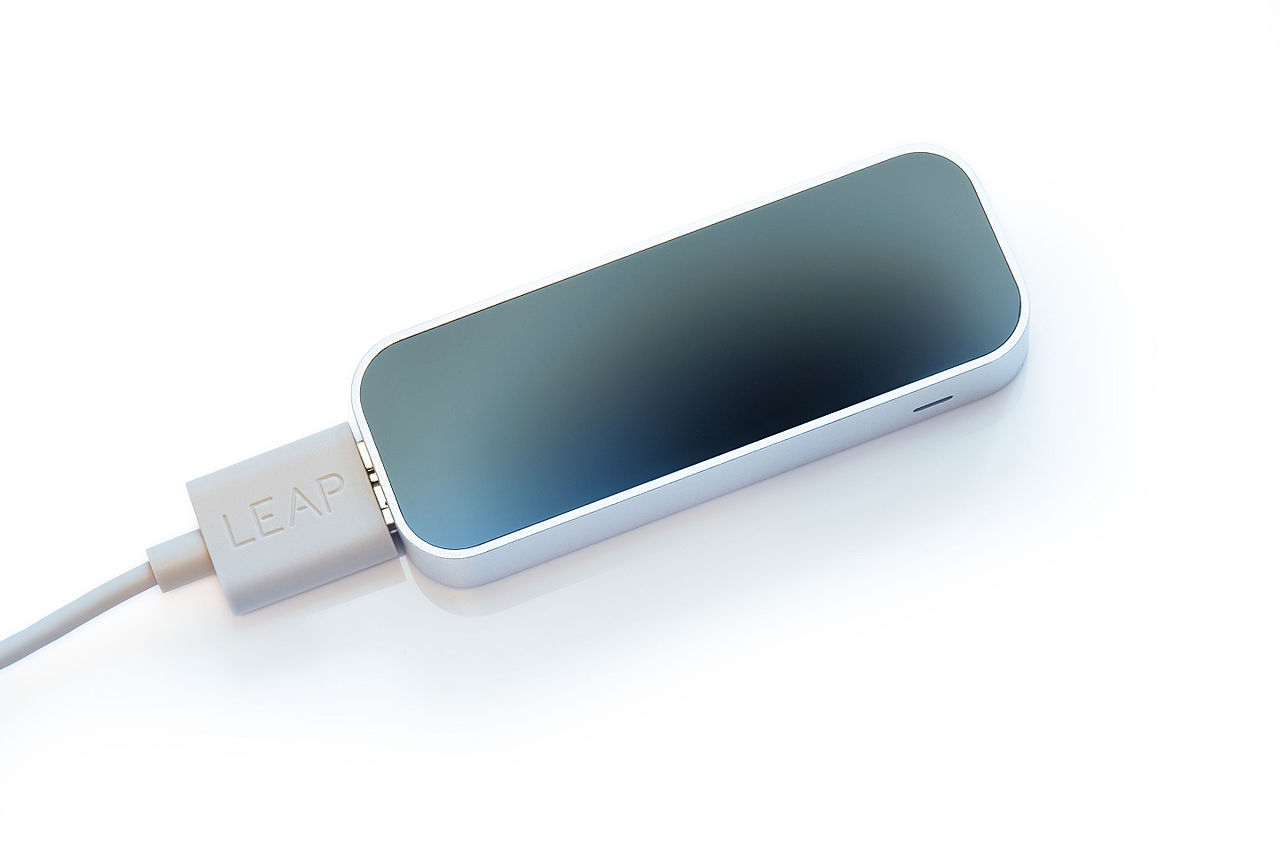
\includegraphics[width=0.9\columnwidth]{figures/LeapMotion_controller}
  \caption{The leapmotion controller}~\label{fig:figure1}
\end{figure}

The \leap{} controller is a device that consists of two stereo cameras which track infrared light with a wavelength of 850 nanometers (allowing it to work even in dark rooms).


The device has a large interaction space, about 0.37 $m^3$. Its range is limited by LED light propagation through space, which is roughly 60cm from the sensor.


After the hardware does its job of recording the images, the software starts doing some heavy mathematical lifting. Despite what most users think, the \leap{} controller uses raw sensor data for tracking, not depth maps.


The \leap{} service is responsible for processing this sensor data. Every application that uses \leap{} has a reference to an implementation of this service, either for \vr or for desktop mode. First, the service removes background objects and compensates for ambient lightning, and then reconstructs a 3D representation of the raw device data.


The tracking layer then extracts information from the 3D representation and feeds these results as frames to a transport protocol. From thereon, each application uses this frames as input.


On June 11, 2018, \leap{} released the latest generation of Orion - version 4. It has been in beta since, but it came with major improvements over the past iterations of \leap{}'s tracking software. These include:

\begin{itemize}
  \item increased range of the sensor from 60 to 80cm
  \item faster hand initialization
  \item better hand pose stability and reliability
  \item more accurate shape and scale for hands
\end{itemize}

\section{REACTIVE EXTENSIONS}

\begin{figure}[H]
  \centering
  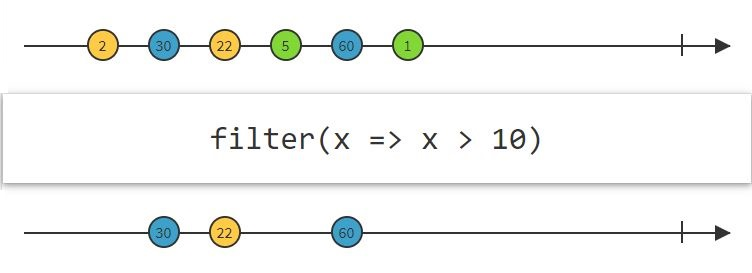
\includegraphics[width=0.9\columnwidth]{figures/RX_filter}
  \caption{Example of a RX operator}~\label{fig:figure2}
\end{figure}
  
ReactiveX is a powerful library for asynchronous and event-based programming. It is an implementation of the observer pattern meant for event-driven programming. It also extends the observer pattern with operators that allow the user to compose sequences declaratively without worrying about low-level concerts (such as mutlithreading and the problems that come with it).


Figure \ref{fig:figure2} shows how an operator works on an observable. In the example, the operator is \textit{filter}. \textit{Filter} takes as input a predicate, a function that maps a value to a boolean (true or false). So, from the source observable [2, 30, 22, 5, 60, 1], by filtering the elemnts greater than 10, we are left with only [30, 22, 60]. Note that the elements are emitted in the same order that they were in the source, almost instantly. The vertical line at the end represents the end of the observable stream. One can attach a callback to that, called \textit{OnComplete}.


The main data structure used by ReactiveX is \textit{Observables}. As stated on their intro page:

\begin{quote}
  You can think of the Observable class as a “push” equivalent to Iterable, which is a “pull.” With an Iterable, the consumer pulls values from the producer and the thread blocks until those values arrive. By contrast, with an Observable the producer pushes values to the consumer whenever values are available. This approach is more flexible, because values can arrive synchronously or asynchronously. (ReactiveX intro)
\end{quote}


The following figures illustrate the resemblance between the iterable and observable.

\begin{figure}[h]
  \centering
  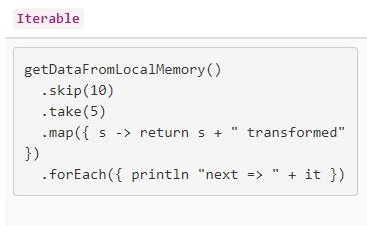
\includegraphics[width=0.9\columnwidth]{figures/RX_iterable}
  \caption{Iterable}~\label{fig:figure3}
\end{figure}

\begin{figure}[h]
  \centering
  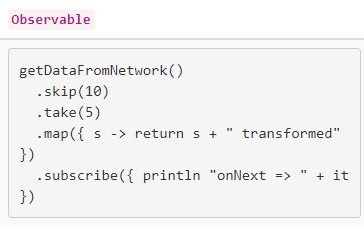
\includegraphics[width=0.9\columnwidth]{figures/RX_observable}
  \caption{Observable}~\label{fig:figure4}
\end{figure}

One might say that the only difference is the call to \textit{subscribe} instead of \textit{forEach}. While, indeed, both of the code snippets produce the same result, the real difference is the data flow.


In the \textit{forEach} example, the thread is blocked until 15 elements arrive from the \textit{getDataFromNetwork} call (first 10 are skipped, then only 5 are processed by the \textit{map}).


In the \textit{subscribe} example, the only delay in the thread's execution is the creation of the observable stream, after which other instructions are executed. When data arrives from the \textit{getDataFromNetwork}, the thread which created the observable is interrupted and data is processed.

\section{LEAPMOTION GESTURES}

The \leap{} API defines mappings for four human body parts:

\begin{itemize}
  \item \textbf{arm} (from elbow to wrist) - has one hand attached
  \item \textbf{hand} - has five fingers attached
  \item \textbf{finger} - has three joints (for attaching objects) and four bones
  \item \textbf{bone}
\end{itemize}

\leap{} offers a variety of gesture detectors already implemented, which can also be combined by the use of a Logic Gate. The logic gate is a higher level detector, combining two or more basic detectors.


As an example, a "thumbs up" gesture would be detected as combination of the following detectors:

\begin{itemize}
  \item Finger Extended Detector - configured to detect a thumb extended and other fingers not extended
  \item Finger Pointing Detector - configured to detect that the thumb is pointing up (\textit{Vector3(0, 0, 1)}) relative to the horizon
  \item And Logic Gate - to combine the other two detectors and have callbacks (C\# scripts) attached to it
\end{itemize}

This approach requires adding three components to a game object and referencing the first two detectors (Finger Extended Detector and Finger Pointing Detector) from the Logic Gate. This can quickly get out of hand when requiring a high number of combined gestures.

\section{FLUENTMOTION GESTURES}

From \leap{}'s human body parts, \fluentmotion{} makes use only of \textbf{hands} and \textbf{fingers}, and defines the following basic gestures.

\subsection{Finger Gestures}
\begin{itemize}
  \item \textit{IsExtended} - selected finger is extended
  \item \textit{IsPointingTo} - selected finger is pointing to a given target (Unity Gameobject or a hand)
  \item \textit{AreExtended} - selected fingers are extended (the others are marked as \textit{don't care}, so they could be extended or not)
\end{itemize}

\subsection{Hand Gestures}

\begin{itemize}
  \item \textit{IsPinching} - hand is pinching (as of Orion 4.4, i.e. \textit{when PinchStrenght > 0.8})
  \item \textit{PalmIsFacing} - palm is facing a given target (can be any object that has a mapping to a Unity \textit{Vector3}) with a given angle tolerance
  \item  \textit{IsFist} - hand is making a fist (i.e. \textit{FistStrenght > 0.8})
  \item \textit{IsMoving} - hand is moving in a given direction (expressed as a Unity \textit{Vector3}) with a given speed (in millimeters per second) and angle tolerance (for the direction) 
  \item \textit{PalmsAreFacing} - both palms are facing a target object or, if no object is given, facing each other with a given angle tolerance
  \item \textit{AreMakingFists} - both hands are making fists
  \item \textit{AreMoving} - both hands are moving in a given direction (\textit{Vector3}) and with a given angle tolerance
\end{itemize}

\fluentmotion{} also supports selecting only some fingers from a hand for extra processing, like checking which is extended and which is not or more complex predicates like finger pointing in a dynamically changing direction.

Besides the already defined gestures, users can create their own gesture detectors by implementing the \textit{IReactiveDetector} or by inheriting from one of its three base implementations: \textit{ReactiveFingerDetector}, \textit{ReactiveHandDetector} or \textit{ReactiveHandsDetector}.

\section{USING FLUENTMOTION}

\subsection{Setup}
After having the \leap{} and \steamvr{} set up, adding \fluentmotion{} to your application is done in two simple steps:

\begin{enumerate}
  \item Add three new empty game objects anywhere in the scene. It is recommended, but not mandatory, to make two of the objects children to the 3\textsuperscript{rd} (as in figure \ref{fig:figure5})
  \begin{figure}[H]
    \centering
    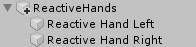
\includegraphics[width=0.9\columnwidth]{figures/FluentMotion_setup}
    \caption{Setting up \fluentmotion{} game objects}~\label{fig:figure5}
  \end{figure}

  \item Attach a \textit{ReactiveHand} script to two of the objects, referencing either the left or the right hand from the LeapRig, and attach a \textit{ReactiveHands} script to the 3\textsuperscript{rd}, referencing the other two \textit{ReactiveHand}s
  \begin{figure}[h]
    \centering
    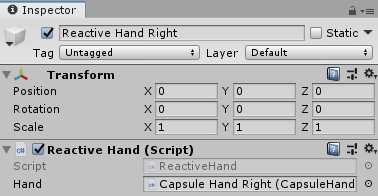
\includegraphics[width=0.9\columnwidth]{figures/FluentMotion_reactive_hand}
    \caption{The \textit{ReactiveHand} script attached to the game object}~\label{fig:figure6}
  \end{figure}
\end{enumerate}

\subsection{Creating Detectors}

To create a detector, simply extend the \textit{ReactiveHandDetector} class in your own script. As an example, the "L" gesture detector - thumb and index are extended, and the others are not.

\begin{figure}[h]
  \centering
  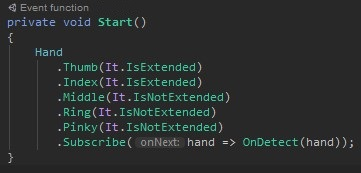
\includegraphics[width=0.9\columnwidth]{figures/FluentMotion_script}
  \caption{The \textit{ReactiveHand} script start function}~\label{fig:figure7}
\end{figure}

The above code is one of the many ways for expressing this detector. Another option is presented in figure \ref{fig:figure8}.

\begin{figure}[H]
  \centering
  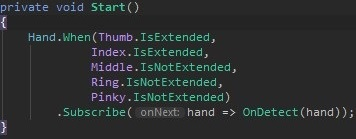
\includegraphics[width=0.9\columnwidth]{figures/FluentMotion_script_alternative}
  \caption{The \textit{ReactiveHand} script start function, using the \textit{When} operator}~\label{fig:figure8}
\end{figure}

Then \textit{When} operator is a very powerful construct available in \fluentmotion{}. It accepts a variable number of predicates, and a combination function for those predicates. If not combination function is given, the default AND is used.


Of course, a mix of the above two methods described in figures \ref{fig:figure7} and \ref{fig:figure8} can be used - say, for when you also want the thumb to point upwards.


The next step is to implement the \textit{OnDetect} method. A possible implementation is shown in figure \ref{fig:figure9}.

\begin{figure}[h]
  \centering
  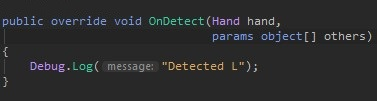
\includegraphics[width=0.9\columnwidth]{figures/FluentMotion_onDetect}
  \caption{\textit{OnDetect} function}~\label{fig:figure9}
\end{figure}

The \textit{params object[] others} are variable arguments - you can pass any extra parameters to this function.


Last, add the script to one of the \textit{ReactiveHand}s in the scene - for example, the right hand.

\begin{figure}[h]
  \centering
  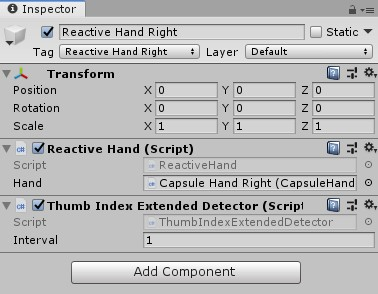
\includegraphics[width=0.9\columnwidth]{figures/FluentMotion_script_attached}
  \caption{Script attached to the right \textit{ReactiveHand}}~\label{fig:figure10}
\end{figure}

The \textit{Interval} field represents the sampling rate expressed in seconds. The sampling rate means how often the same gesture should be detected. The field is of type \textbf{double}, so values less than 1 second can be set. The default value is 500ms (0.5 seconds).

% \begin{table}
%   \centering
%   \begin{tabular}{l r r r}
%     % \toprule
%     & & \multicolumn{2}{c}{\small{\textbf{Test Conditions}}} \\
%     \cmidrule(r){3-4}
%     {\small\textit{Name}}
%     & {\small \textit{First}}
%       & {\small \textit{Second}}
%     & {\small \textit{Final}} \\
%     \midrule
%     Marsden & 223.0 & 44 & 432,321 \\
%     Nass & 22.2 & 16 & 234,333 \\
%     Borriello & 22.9 & 11 & 93,123 \\
%     Karat & 34.9 & 2200 & 103,322 \\
%     % \bottomrule
%   \end{tabular}
%   \caption{Table captions should be placed below the table. We
%     recommend table lines be 1 point, 25\% black. Minimize use of
%     table grid lines.}~\label{tab:table1}
% \end{table}


% BALANCE COLUMNS
%\balance{}

\bibliographystyle{SIGCHI-Reference-Format}
\bibliography{sample}

\end{document}

%%% Local Variables:
%%% mode: latex
%%% TeX-master: t
%%% End:
